% !TEX TS-program = lualatex
%\documentclass[handout]{beamer}
\documentclass{beamer}
\input{../common/misomva}
\newcommand{\misoclasstinytitleslide}{Partially based on material by:  Ulrike von Luxburg, \\[-1em] Gary Miller, Doyle \& Schnell, Daniel Spielman}
\newcommand{\misoclassdate}{}
\usetikzlibrary{graphs}

\begin{document}
% Topic-specific title slide

\newcommand{\topictitle}{Spectral Clustering: RatioCut \& NCut}

\newcommand{\topicsubtitle}{Relaxation \& Approximation Algorithms}

\MakeTopicSlide

%%%%%%%%%%%%%%%%%%%%%%%%%%%%%%%%%%%%%%%%%%%%%%%%%%%%%%%%%%%%
% Detailed relaxation steps (from relaxation-ratiocut.tex frames 1-3)
\begin{frame}
\frametitle{Spectral Clustering: Relaxing Balanced Cuts}
\begin{block}{Relaxation for (simple) balanced cuts for 2 sets}
\[\min_{A,B} {\rm cut}(A,B) \quad {\rm s.t.} \quad  |A|=|B|\]
\end{block}
\bigskip \pause
Graph function $\bff$ for cluster membership\pause : 
$ f_i = 
\begin{cases}
1 & \mbox{if } V_i \in A, \\
-1 & \mbox{if } V_i \in B. \\ 
\end{cases}$
\bigskip \pause
\questionbox{What it is the cut value with this definition?}
\[
{\rm cut}(A,B) 
= \pause \sum_{i\in A, j\in B} w_{i,j}
= \tfrac14 \sum_{i,j}  w_{i,j} (f_i-f_j)^2
= \tfrac12 \bff\transpose \bL \bff
\]
\pause
\questionbox{What is the relationship with the \gcol{smoothness} of a graph function?}

\end{frame}
\begin{frame}
\frametitle{Spectral Clustering: Relaxing Balanced Cuts}
\[
{\rm cut}(A,B) 
= \sum_{i\in A, j\in B} w_{i,j}
= \tfrac14 \sum_{i,j}  w_{i,j} (f_i-f_j)^2
= \tfrac12 \bff\transpose \bL \bff
\]
\pause
$|A| = |B| \implies \sum_i f_i = \pause 0 \implies \pause \bff \perp \bOne_\nodes$ 
\\ \bigskip 
$\|\bff\| = \pause \sqrt{\nodes}$ \pause

\begin{center}
\begin{block}{\centering objective function of spectral clustering}
\[
\min_{\bff} \bff\transpose \bL \bff \quad {\rm s.t.} 
\quad f_i = \pm 1,
\quad \bff \perp \bOne_\nodes, 
\quad \|\bff\| =  \sqrt{\nodes}
\]
\end{block}
\bigskip
 \pause 
Still NP hard :( \pause  $\quad \to \quad$
\yellbox{Relax even further!} \\
\pause \bigskip 
\tikz[baseline]
\node [cross out,draw=red,anchor=text] {$f_i = \pm 1$};
$\quad \to \quad f_i \in \R$

\end{center}
\end{frame}
\begin{frame}
\frametitle{Spectral Clustering: Relaxing Balanced Cuts}
\begin{block}{\centering objective function of spectral clustering}
\[
\min_{\bff} \bff\transpose \bL \bff \quad {\rm s.t.} 
\quad f_i \in \R,
\quad \bff \perp \bOne_\nodes, 
\quad \|\bff\| =  \sqrt{\nodes}
\]
\end{block}


\only<2,3 | handout:1>{
\begin{block}{\centering Rayleigh-Ritz theorem}
If $\lambda_1 \leq \dots \leq \lambda_\nodes$ are the eigenvalues of real symmetric $\bL$ then
\begin{align*}
 \lambda_1 &= \min_{\bx \ne 0} \frac{\bx\transpose\bL \bx}{\bx\transpose\bx} = \min_{\bx\transpose\bx=1}\bx\transpose\bL \bx\\
 \lambda_\nodes &= \max_{\bx \ne 0} \frac{\bx\transpose\bL \bx}{\bx\transpose\bx} = \max_{\bx\transpose\bx=1}\bx\transpose\bL \bx 
\end{align*}
\end{block}
$\frac{\bx\transpose\bL \bx}{\bx\transpose\bx} \equiv$ \gcol{Rayleigh quotient}
}

\only<3| handout:1>{ \begin{center}\questionbox{How can we use it?} \end{center} }
 
 \only<4| handout:2>{
 \begin{block}{\centering Generalized Rayleigh-Ritz theorem (Courant-Fischer-Weyl)}
 If $\lambda_1 \leq \dots \leq \lambda_\nodes$ are the eigenvalues of real symmetric $\bL$ 
 and $\bv_1, \dots, \bv_\nodes$ the corresponding orthogonal eigenvectors, then for $k = 1:\nodes-1$
 \begin{align*}
  \lambda_{k+1} &= \min_{\bx \ne 0, \bx \perp \bv_1, \dots \bv_k} \frac{\bx\transpose\bL \bx}{\bx\transpose\bx} 
      = \min_{\bx\transpose\bx=1, \bx \perp \bv_1, \dots \bv_k}\bx\transpose\bL \bx\\
  \lambda_{\nodes-k} &= \max_{\bx \ne 0, \bx \perp \bv_n, \dots \bv_{\nodes-k+1}} \frac{\bx\transpose\bL \bx}{\bx\transpose\bx} 
      = \max_{\bx\transpose\bx=1, \bx \perp \bv_\nodes, \dots \bv_{\nodes-k+1}}\bx\transpose\bL \bx 
 \end{align*}
 \end{block}
 }

\end{frame}
%%%%%%%%%%%%%%%%%%%%%%%%%%%%%%%%%%%%%%%%%%%%%%%%%%%%%%%%%%%%
% Final objective and solution (from relaxation-ratiocut.tex frame 4)
\begin{frame}
\frametitle{Spectral Clustering: Relaxing Balanced Cuts}
\begin{block}{\centering objective function of spectral clustering}
\[
\min_{\bff} \bff\transpose \bL \bff \quad {\rm s.t.} 
\quad f_i \in \R,
\quad \bff \perp \bOne_\nodes, 
\quad \|\bff\| =  \sqrt{\nodes}
\]
\end{block}

Solution: \pause \emphcol{second eigenvector}  \questionbox{How do we get the clustering?}
\\ \smallskip \pause 
The solution may not be integral. \questionbox{What to do?}
\\ \smallskip \pause 
\[
{\rm cluster}_i = 
\begin{cases}
1 & \mbox{if } f_i \geq 0, \\
-1 & \mbox{if } f_i < 0. \end{cases}
\]
\\ \pause 
Works but this heuristics is often too simple. \pause In practice, cluster $\bff$ using $k$-means to get 
$\{C_i\}_{i}$ and assign:
\\  \pause 
\[
{\rm cluster}_i = 
\begin{cases}
1 & \mbox{if } i \in C_1, \\
-1 & \mbox{if } i \in C_{-1}. \end{cases}
\]
\end{frame}
%%%%%%%%%%%%%%%%%%%%%%%%%%%%%%%%%%%%%%%%%%%%%%%%%%%%%%%%%%%%
% RatioCut approximation (from relaxation-ratiocut.tex frames 5-6)
\begin{frame}
\frametitle{Spectral Clustering: Approximating RatioCut}
\begin{center}
 \yellbox{Wait, but we did not care about approximating mincut!}
\end{center}
\pause
\begin{block}{RatioCut}
\[{\rm RatioCut}(A,B)= \sum_{i\in A, j\in B} w_{ij} \left( \frac{1}{|A|} + \frac{1}{|B|} \right) \]
\end{block}
\pause
Define graph function $\bff$ for cluster membership of RatioCut\pause : 
\[ f_i = 
\begin{cases}
\sqrt{\frac{|B|}{|A|}} & \mbox{if } V_i \in A, \\
- \sqrt{\frac{|A|}{|B|}} & \mbox{if } V_i \in B. \\ 
\end{cases} \]
 \pause
\[
\bff\transpose \bL \bff 
= \tfrac12  \sum_{i,j}  w_{i,j} (f_i-f_j)^2
= \pause (|A|+|B|) {\rm RatioCut}(A,B)
\]
\end{frame}
%%%%%%%%%%%%%%%%%%%%%%%%%%%%%%%%%%%%%%%%%%%%%%%%%%%%%%%%%%%%

\begin{frame}
\frametitle{Spectral Clustering: Approximating RatioCut}
Define graph function $\bff$ for cluster membership of RatioCut\pause : 
\[ f_i = 
\begin{cases}
\sqrt{\frac{|B|}{|A|}} & \mbox{if } V_i \in A, \\
- \sqrt{\frac{|A|}{|B|}} & \mbox{if } V_i \in B. \\ 
\end{cases} \]
 \pause
\[
\sum_{i}  f_i = \pause 0
\]
\[
\sum_{i}  f_i^2 = \pause \nodes
\]
\pause
\begin{block}{\centering objective function of spectral clustering (same - it's magic!)	}
\[
\min_{\bff} \bff\transpose \bL \bff \quad {\rm s.t.} 
\quad f_i \in \R,
\quad \bff \perp \bOne_\nodes, 
\quad \|\bff\| =  \sqrt{\nodes}
\]
\end{block}
\end{frame}
%%%%%%%%%%%%%%%%%%%%%%%%%%%%%%%%%%%%%%%%%%%%%%%%%%%%%%%%%%%%
% NCut approximation (from ratiocut-ncut.tex frames 4-6)
\begin{frame}
\frametitle{Spectral Clustering: Approximating NCut}
\begin{block}{Normalized Cut}
\[{\rm NCut}(A,B)= \sum_{i\in A, j\in B} w_{ij} \left( \frac{1}{{\rm vol}(A)} + \frac{1}{{\rm vol}(B)} \right) \]
\end{block}
\pause
Define graph function $\bff$ for cluster membership of NCut: 
\[ f_i = 
\begin{cases}
\sqrt{\frac{{\rm vol}(B)}{{\rm vol}(A)}} & \mbox{if } V_i \in A, \\
- \sqrt{\frac{{\rm vol}(A)}{{\rm vol}(B)}} & \mbox{if } V_i \in B.
\end{cases} \]
 \pause \vspace{-1em}
\[
(\bD\bff)\transpose\bOne_n = 0 \pause \qquad  
\bff\transpose \bD \bff =  {\rm vol}(\nodeset) \pause \qquad  
\bff\transpose \bL \bff = {\rm vol}(\nodeset) {\rm NCut}(A,B)
\]
\pause \vspace{-1em}
\begin{block}{\centering objective function of spectral clustering (NCut)}
\[ 
\min_{\bff} \bff\transpose \bL \bff \quad {\rm s.t.} 
\quad f_i \in \R,
\quad \bD\bff \perp \bOne_\nodes, 
\quad \bff\transpose \bD \bff  = {\rm vol}(\nodeset)
\]
\end{block}
\end{frame}
%%%%%%%%%%%%%%%%%%%%%%%%%%%%%%%%%%%%%%%%%%%%%%%%%%%%%%%%%%%%
%%%%%%%%%%%%%%%%%%%%%%%%%%%%%%%%%%%%%%%%%%%%%%%%%%%%%%%%%%%%
\begin{frame}
\frametitle{Spectral Clustering: Approximating NCut}
\begin{block}{\centering objective function of spectral clustering (NCut)}
\[
\min_{\bff} \bff\transpose \bL \bff \quad {\rm s.t.} 
\quad f_i \in \R,
\quad \bD\bff \perp \bOne_\nodes, 
\quad \bff\transpose \bD \bff  = {\rm vol}(\nodeset)
\]
\end{block}
\questionbox{Can we apply Rayleigh-Ritz now?} \, \pause Define $\bw = \bD^{1/2}\bff$ \pause
\begin{block}{\centering objective function of spectral clustering (NCut)}
\[
\min_{\bw} \bw \transpose \bD^{-1/2} \bL \bD^{-1/2}\bw \quad {\rm s.t.} 
\quad w_i \in \R,
\bw \perp \bD^{1/2}\bOne_\nodes, 
\|\bw\|^2  = {\rm vol}(\nodeset)
\]
\end{block} \pause

\begin{block}{\centering objective function of spectral clustering (NCut)}
\[  
\min_{\bw} \bw \transpose  \bL_{\rm sym} \bw \quad {\rm s.t.} 
\quad w_i \in \R,
\quad \bw \perp \bv_{1, \bL_{\rm sym}}, 
\quad \|\bw\|^2  = {\rm vol}(\nodeset)
\]
\end{block} 
\end{frame}
%%%%%%%%%%%%%%%%%%%%%%%%%%%%%%%%%%%%%%%%%%%%%%%%%%%%%%%%%%%%
%%%%%%%%%%%%%%%%%%%%%%%%%%%%%%%%%%%%%%%%%%%%%%%%%%%%%%%%%%%%
\begin{frame}
\frametitle{Spectral Clustering: Approximating NCut}
\begin{block}{\centering objective function of spectral clustering (NCut)}
\vspace{-1em}	
\[  
\min_{\bw} \bw \transpose  \bL_{\rm sym} \bw \quad {\rm s.t.} 
\quad w_i \in \R,
\quad \bw \perp \bv_{1, \bL_{\rm sym}}, 
\quad \|\bw\|  = {\rm vol}(\nodeset)
\]
\end{block} \pause \bigskip
\questionbox{Solution by Rayleigh-Ritz?} \, 
\pause $\bw = \bv_{2, \bL_{\rm sym}}$
\pause $\bff =  \pause \bD^{-1/2}\bw$
\pause \\ \bigskip
\yellbox{$\bff$ is a the second eigenvector of $\bL_{\rm rw}$ !} 
\pause \\ \bigskip
\textbf{tl;dr:} Get the second eigenvector of $\bL$/$\bL_{\rm rw}$  for RatioCut/NCut. 
\pause \\ \bigskip
{\tiny demo: \url{https://dominikschmidt.xyz/spectral-clustering-exp/}}\\

\end{frame}
%%%%%%%%%%%%%%%%%%%%%%%%%%%%%%%%%%%%%%%%%%%%%%%%%%%%%%%%%%%
% Approximation example (from ratiocut-ncut.tex frame 7)
\begin{frame}
\frametitle{Spectral Clustering: Approximation}
These are all approximations.  \questionbox{How bad can they be?} 
\pause \\ \bigskip
\onslide<handout:0>{\notecol{%
Pretty bad.}}
\pause \, Example: cockroach graphs
\begin{center}
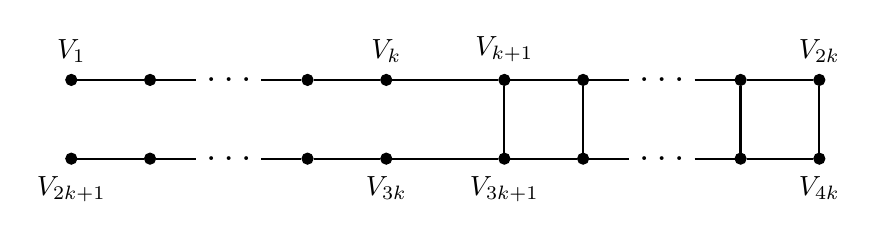
\begin{tikzpicture}[scale=1.0]
    \tikzstyle{vertex}=[circle, draw=black, fill=black, inner sep=0pt, minimum size=4pt]
    \tikzstyle{dots}=[font=\Large]

    % === LEFT PART (Legs) ===
    % V1 / V2k+1
    \node[vertex] (t1) at (0, 1) {};
    \node[vertex] (b1) at (0, 0) {};
    \node[above=0.1cm] at (t1) {$V_1$};
    \node[below=0.1cm] at (b1) {$V_{2k+1}$};

    % Node
    \node[vertex] (t2) at (1, 1) {};
    \node[vertex] (b2) at (1, 0) {};
    
    % Dots
    \node[dots] (td1) at (2, 1) {$\dots$};
    \node[dots] (bd1) at (2, 0) {$\dots$};
    
    % Node
    \node[vertex] (t3) at (3, 1) {};
    \node[vertex] (b3) at (3, 0) {};
    
    % Vk / V3k
    \node[vertex] (tk) at (4, 1) {};
    \node[vertex] (bk) at (4, 0) {};
    \node[above=0.1cm] at (tk) {$V_k$};
    \node[below=0.1cm] at (bk) {$V_{3k}$};

    % Edges Left
    \draw[thick] (t1) -- (t2) -- (td1) -- (t3) -- (tk);
    \draw[thick] (b1) -- (b2) -- (bd1) -- (b3) -- (bk);


    % === CONNECTION ===
    % Vk+1 / V3k+1
    \node[vertex] (tk1) at (5.5, 1) {};
    \node[vertex] (bk1) at (5.5, 0) {};
    \node[above=0.1cm] at (tk1) {$V_{k+1}$};
    \node[below=0.1cm] at (bk1) {$V_{3k+1}$};
    
    % Connection Edges
    \draw[thick] (tk) -- (tk1);
    \draw[thick] (bk) -- (bk1);


    % === RIGHT PART (Ladder) ===
    % Vertical edge at start of ladder
    \draw[thick] (tk1) -- (bk1);
    
    % Node
    \node[vertex] (t4) at (6.5, 1) {};
    \node[vertex] (b4) at (6.5, 0) {};
    \draw[thick] (t4) -- (b4); % Vertical
    
    % Dots
    \node[dots] (td2) at (7.5, 1) {$\dots$};
    \node[dots] (bd2) at (7.5, 0) {$\dots$};
    % Vertical dots? Usually not drawn, but ladder structure implies it.
    
    % Node
    \node[vertex] (t5) at (8.5, 1) {};
    \node[vertex] (b5) at (8.5, 0) {};
    \draw[thick] (t5) -- (b5); % Vertical
    
    % V2k / V4k
    \node[vertex] (t2k) at (9.5, 1) {};
    \node[vertex] (b2k) at (9.5, 0) {};
    \node[above=0.1cm] at (t2k) {$V_{2k}$};
    \node[below=0.1cm] at (b2k) {$V_{4k}$};
    \draw[thick] (t2k) -- (b2k); % Vertical

    % Edges Right
    \draw[thick] (tk1) -- (t4) -- (td2) -- (t5) -- (t2k);
    \draw[thick] (bk1) -- (b4) -- (bd2) -- (b5) -- (b2k);

\end{tikzpicture}
\end{center}
\pause  \bigskip
No efficient approximation exist. Other relaxations possible. 

{\tiny \url{https://www.cs.cmu.edu/~glmiller/Publications/Papers/GuMi95.pdf}}
\end{frame}

%%%%%%%%%%%%%%%%%%%%%%%%%%%%%%%%%%%%%%%%%%%%%%%%%%%%%%%%%%%%
% 1D Example (from ratiocut-ncut.tex frame 8)
\begin{frame}
\frametitle{Spectral Clustering: 1D Example}
 \begin{center}
\onslide<5>{\gcol{Elbow rule/EigenGap heuristic} for number of clusters}\\
\bigskip
\includegraphics<1>[width=\columnwidth]{../img/luxburgh-example-number_1_transparent}%
\includegraphics<2>[width=\columnwidth]{../img/luxburgh-example-number_2_transparent}%
\includegraphics<3>[width=\columnwidth]{../img/luxburgh-example-number_3_transparent}%
\includegraphics<4-5>[width=\columnwidth]{../img/luxburgh-example-number_4_transparent}%
\\
{\tiny Source: von Luxburg (2007)}
\end{center}
\end{frame}
%%%%%%%%%%%%%%%%%%%%%%%%%%%%%%%%%%%%%%%%%%%%%%%%%%%%%%%%%%%%



\MakeLastSlide
\end{document}
